% Presentation Beamer
% Characteristics:
% -- Several Themes
% -- 

%%%%%%%%%%%%%%%%%%%%%%
%%%%%%%%%%%%%%%%%%%%%%
%%% Document Start %%%
%%%%%%%%%%%%%%%%%%%%%%
%%%%%%%%%%%%%%%%%%%%%%

\documentclass{beamer}

%%%%%%%%%%%%%%%%%%%%%%%%
%%% General Settings %%%
%%%%%%%%%%%%%%%%%%%%%%%%

%%% Packages %%%
\usepackage{verbatim}
\usepackage{graphicx}
\usepackage{subfig}
\usepackage{float}
\usepackage[ruled,linesnumbered]{algorithm2e}

%%% Definitions %%%

%%% Theme Selection %%%
%\usetheme{AnnArbor}
\usetheme{Antibes}
%\usetheme{Bergen}
%\usetheme{Berkeley}
%\usetheme{Berlin}
%\usetheme{Boadilla}
%\usetheme{boxes}
%\usetheme{CambridgeUS}
%\usetheme{Copenhagen}
%\usetheme{Darmstadt}
%\usetheme{default}
%\usetheme{Frankfurt}
%\usetheme{Goettingen}
%\usetheme{Hannover}
%\usetheme{Ilmenau}
%\usetheme{JuanLesPins}
%\usetheme{Luebeck}
%\usetheme{Madrid}
%\usetheme{Malmoe}
%\usetheme{Marburg}
%\usetheme{Montpellier}
%\usetheme{PaloAlto}
%\usetheme{Pittsburgh}
%\usetheme{Rochester}
%\usetheme{Singapore}
%\usetheme{Szeged}
%\usetheme{Warsaw}

%%% PDF Subject Catalog %%%
% - This is only inserted into the PDF information catalog. Can be left
% out.
\subject{Reinforcement Learning}

%%% Institution Logo %%% - Optional
% If you have a file called "university-logo-filename.xxx", where xxx
% is a graphic format that can be processed by latex or pdflatex,
% resp., then you can add a logo as follows:
\pgfdeclareimage[height=0.5cm]{university-logo}{university-logo-filename}
\logo{\pgfuseimage{university-logo}}

%%%%%%%%%%%%%%%%%%%%%%%%%%
%%% Presentation Cover %%%
%%%%%%%%%%%%%%%%%%%%%%%%%%

%%% Presentation Title %%%
\title{Defenses against Adversarial Examples}

%%% Subtitle %%% - Optional
%\subtitle{and Other RL Methods}

%%% Presentation Authors %%%%
% - Give the names in the same order as the appear in the paper.
% - Use the \inst{?} command only if the authors have different
%   affiliation.
\author{Keller Jordan$^1$, Rene Gutierrez$^2$, Brett Gohre$^3$}

%%% Author Affiliation %%% - Optional
% - Use the \inst command only if there are several affiliations.
% - Keep it simple, no one is interested in your street address.
\institute[University of California Santa Cruz]
{
\inst{1}%
Department of Computer Science \\
UCSC
\and
\inst{2}%
Department of Applied Mathematics \& Statistics \\
UCSC
\and
\inst{3}%
Department of Physical \& Biological Sciences \\
UCSC
}


%%% Conference Name and Information %%% - Optional
% - Either use conference name or its abbreviation.
% - Not really informative to the audience, more for people (including
%   yourself) who are reading the slides on-line
\date{CMPS290, Winter 2018}

%%% Table of Contents %%% - Optional
% Delete this, if you do not want the table of contents to pop up at
% the beginning of each subsection:
\begin{comment}
\AtBeginSubsection[]
{
\begin{frame}<beamer>{Outline}
\tableofcontents[currentsection,currentsubsection]
\end{frame}
}
\end{comment}

%%%%%%%%%%%%%%%%%%%%%%%%%%%%
%%% Presentation Content %%%
%%%%%%%%%%%%%%%%%%%%%%%%%%%%

\begin{document}
	
	%%% Title Page %%%
	\begin{frame}
		\titlepage
	\end{frame}
	
	
	%%% Outline %%% - Optional
	% - You might wish to add the option [pausesections]
	% - Section and subsections will appear in the presentation overview
	% and table of contents.
	%\begin{frame}{Outline}
	%  \tableofcontents
	%\end{frame}
	
	%%% Body %%%
	\graphicspath{{figures/}}
	
	\section*{Introduction}
	
	\section*{Optimizer Robustness}
	
	\begin{frame}{Optimizer Robustness}
		\begin{block}{We studied:}
			\begin{itemize}
				\item Vanilla gradient descent
				\item EG plus/minus
			\end{itemize}
		\end{block}
	\end{frame}
	
	\begin{frame}{Procedure}
		\begin{itemize}
			\item Train same model with GD and EG$\pm$ on MNIST
			\item Model is fully-connected 784-100-10
			\item Run non-targeted adversarial attack until fooled on subset
			\item Attacks were gradient ascent (GA) and fast gradient sign method (FGS)
			\item Average added noise for each class
			\item Compare results between models
		\end{itemize}
	\end{frame}
	
	\begin{frame}{Attack Difficulty}
		\begin{block}{Number of iterations to fool network}
			\begin{center}
				\begin{tabular}{| l | l | l |}
					\hline
					Method / Optimizer & SGD & EG \\ \hline
					Gradient Ascent & $60.9 (\pm 32.3)$ & $85.1 (\pm 40.5)$ \\ \hline
					Fast Gradient Sign & $52.0 (\pm 26.1)$ & $91.0 (\pm 43.5)$ \\ \hline
				\end{tabular}
			\end{center}
		\end{block}
		A network is ``fooled" when its prediction changes (untargeted attack)
	\end{frame}
	
	\begin{frame}{Average Perturbation}
		\centering
		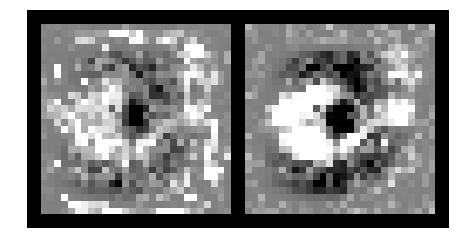
\includegraphics[width=\textwidth]{avg_attack_3}
		
		SGD (left), EG$\pm$ (right)
	\end{frame}
	
	\begin{frame}{Transferability Results}
		\begin{block}{Transferability of attacks between optimizers}
			\begin{center}
				\begin{tabular}{| l | l | l |}
					\hline
					Method / Src$\rightarrow$Dst & SGD$\rightarrow$EG & EG$\rightarrow$SGD  \\ \hline
					Gradient Ascent & 67.4\% & 99.0\% \\ \hline
					Fast Gradient Sign & 88.2\% & 99.8\% \\ \hline
				\end{tabular}
			\end{center}
		\end{block}
		Iterations held constant at 200
	\end{frame}
	
	\begin{frame}{Notes}
		\begin{itemize}
			\item FGS looks better to humans, worse for MSE
			\item GA better at revealing structure of model since cares about strength of change
			\item Next step: should try L1 norm weights to see difference
		\end{itemize}
	\end{frame}

	\section*{Reconstruction as a Defense}
	
	\begin{frame}{Reconstruction as a Defense}
		\begin{block}{How to get recon err?}
			Need some way to reconstruct image
			
			Could use encoder/decoder
			
			I went with capsule network
		\end{block}
	\end{frame}
	
	\begin{frame}{Capsule Network Refresher}
		details about reconstruction network and capsnet
	\end{frame}
	
	\begin{frame}{Results}
		\centering
		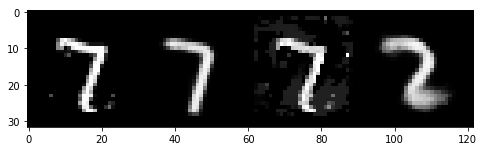
\includegraphics[width=\textwidth]{recon-fig1}
	\end{frame}
	
	\begin{frame}{CIFAR10}
		Capsules are not there yet.
		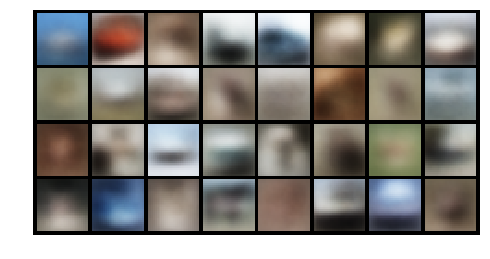
\includegraphics[width=\textwidth]{cifar_recon}
	\end{frame}
	
	\begin{frame}{ROC Curve}
		\centering
		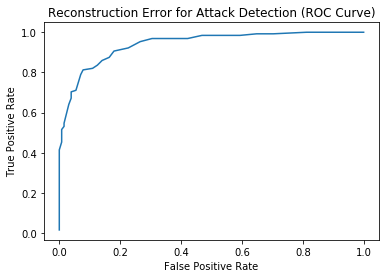
\includegraphics[width=10cm]{mse_roc}
	\end{frame}
	
	
	% All of the following is optional and typically not needed.
	\begin{comment}
	\appendix
	\section<presentation>*{\appendixname}
	\subsection<presentation>*{For Further Reading}
	
	\begin{frame}[allowframebreaks]
	\frametitle<presentation>{For Further Reading}
	
	\begin{thebibliography}{10}
	
	\beamertemplatebookbibitems
	% Start with overview books.
	
	\bibitem{Author1990}
	A.~Author.
	\newblock {\em Handbook of Everything}.
	\newblock Some Press, 1990.
	
	
	\beamertemplatearticlebibitems
	% Followed by interesting articles. Keep the list short. 
	
	\bibitem{Someone2000}
	S.~Someone.
	\newblock On this and that.
	\newblock {\em Journal of This and That}, 2(1):50--100,
	2000.
	\end{thebibliography}
	
	\end{frame}
	
	\begin{itemize}
	\item
	Outlook
	\begin{itemize}
	\item
	Something you haven't solved.
	\item
	Something else you haven't solved.
	\end{itemize}
	\end{itemize}
	
	\end{comment}
	
\end{document}